
plane tree is compared with sota mesh compression - proven by my paper published and in terms of compressing 3d reconstructions we compare it to the common OT representation \\

Experiments reveal the Plane-Tree outperforms the original octree and outperforms some state of the art transform methods at low-bitrates. We compare our method with several state of the art algorithms which correspond to transform based methods \cite{Khodakovsky00Progressive,Bayazit103DMesh} and low-bitrate codecs \cite{Peng10Feature}. To compare algorithms quantitatively, we employ rate distortion graphs. Since our algorithm is lossy, this indicates the amount of distortion (in the decoded model compared with the original) given a particular bitrate. To measure distortion, we employ the mean error and root mean squared error, to measure bitrate we use the number of bits per vertex. All measurements are scaled by the main diagonal of the input model. We also provide qualitative results showing the effectiveness of our method. \\

In experiments we use 4 models which are popular amongst researchers in the area. These models are chosen both because they are readily available and because there are available results for these models generated by other state of the art methods. Figure \ref{fig:MODSUSED} shows each model along with its reference name and number of vertices. \\


\begin{figure}[t!] 
        \centering
        \begin{subfigure}[b]{2.8in}
                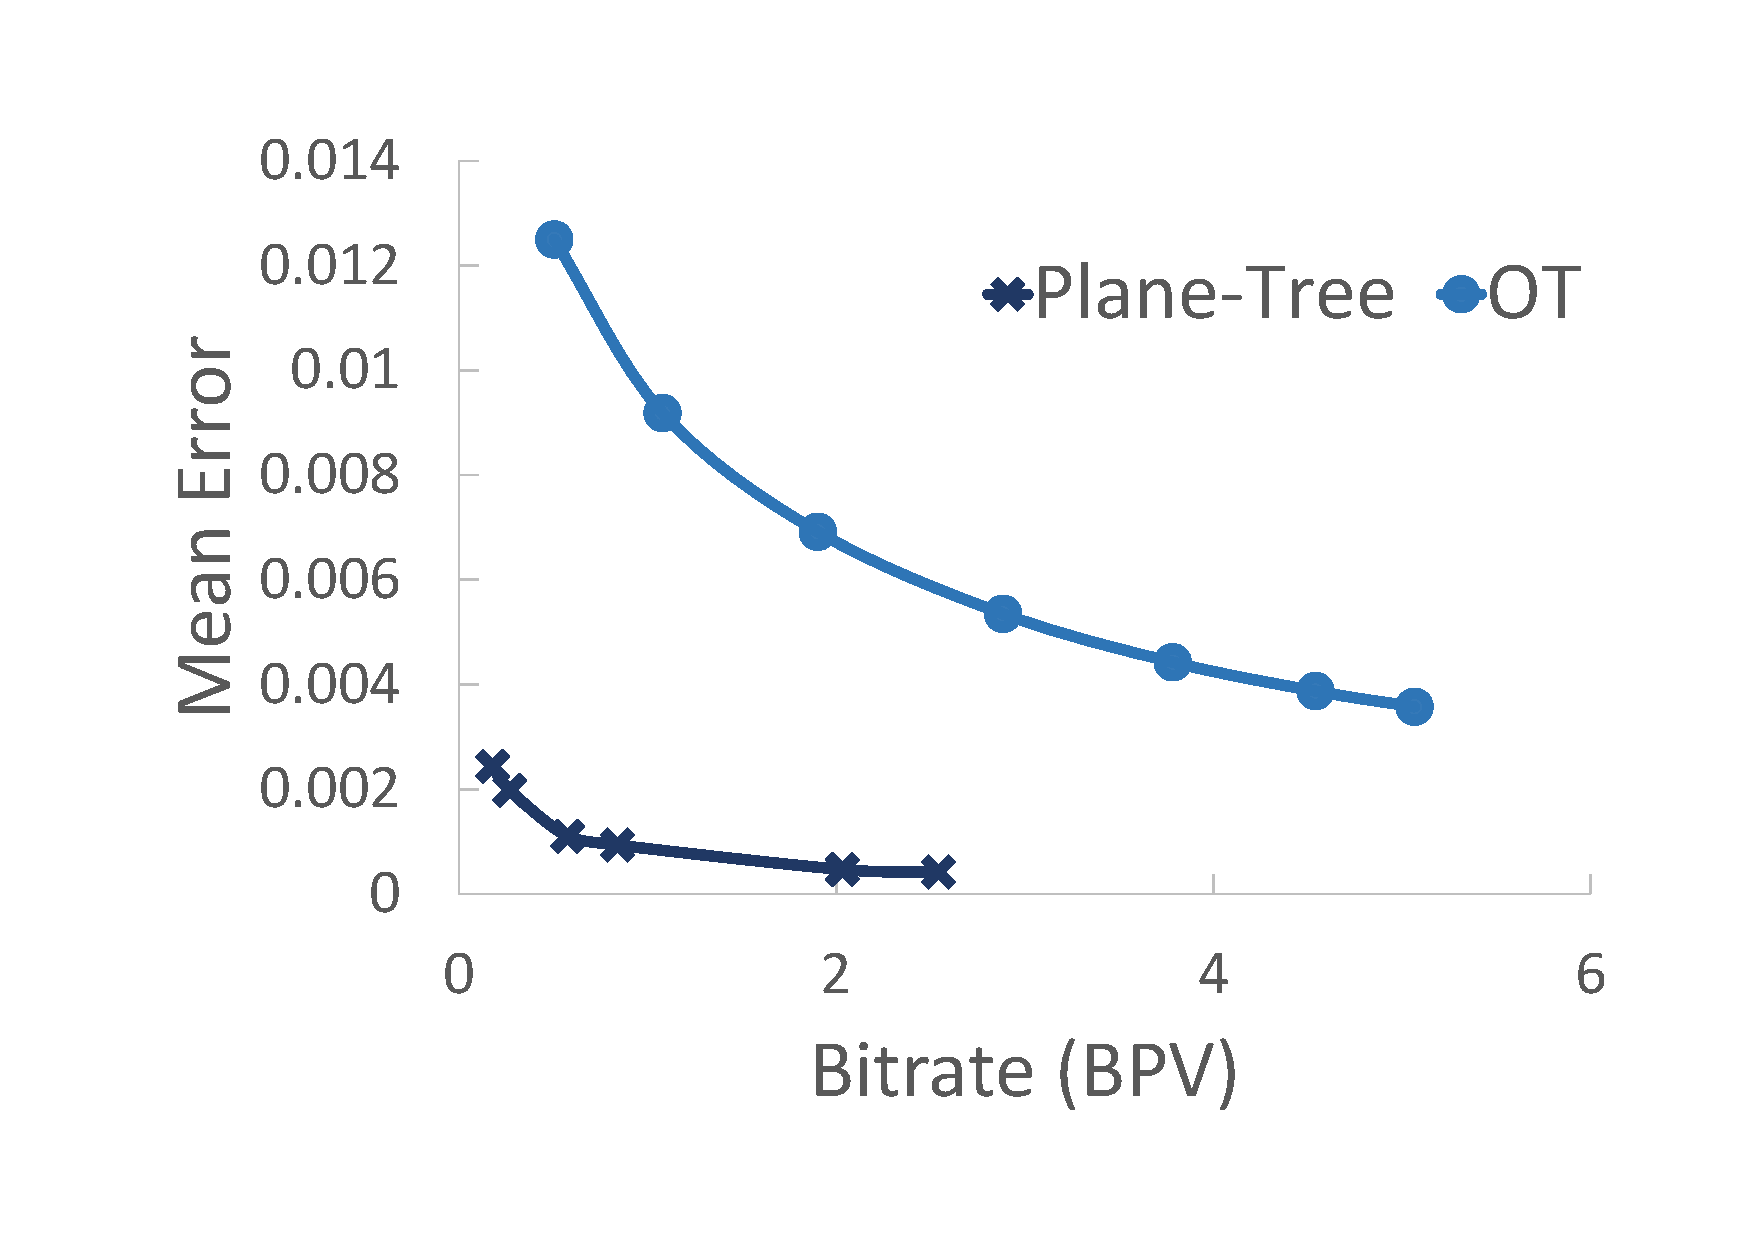
\includegraphics[width=2.5in]{images/results/compression/OTbunny}
                \caption{Bunny Model}
                \label{fig:OG_BUNNY}
        \end{subfigure}
        
        \begin{subfigure}[b]{2.8in}
                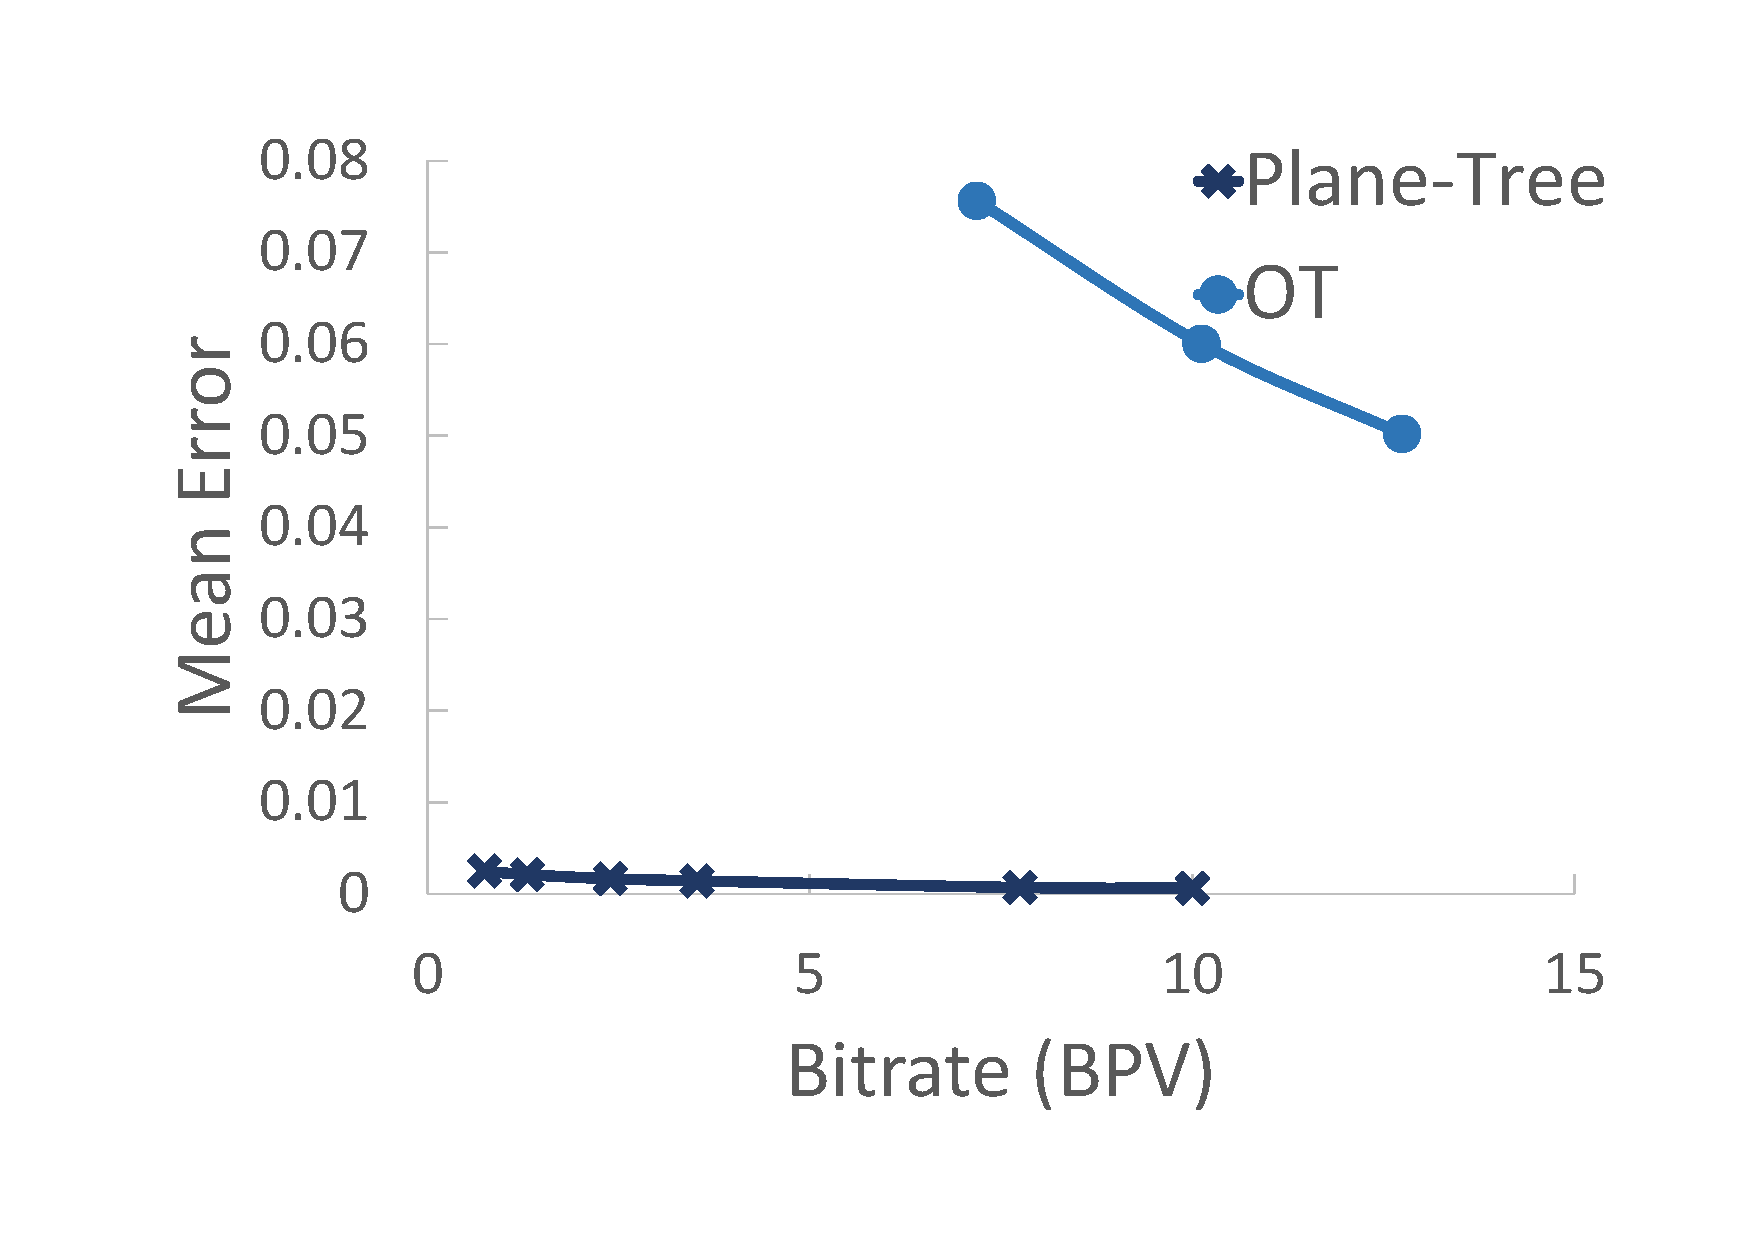
\includegraphics[width=2.5in]{images/results/compression/OTFandisk}
                \caption{Fandisk Model}
                \label{fig:OG_FANDISK}
        \end{subfigure}
        
        \begin{subfigure}[b]{2.8in}
                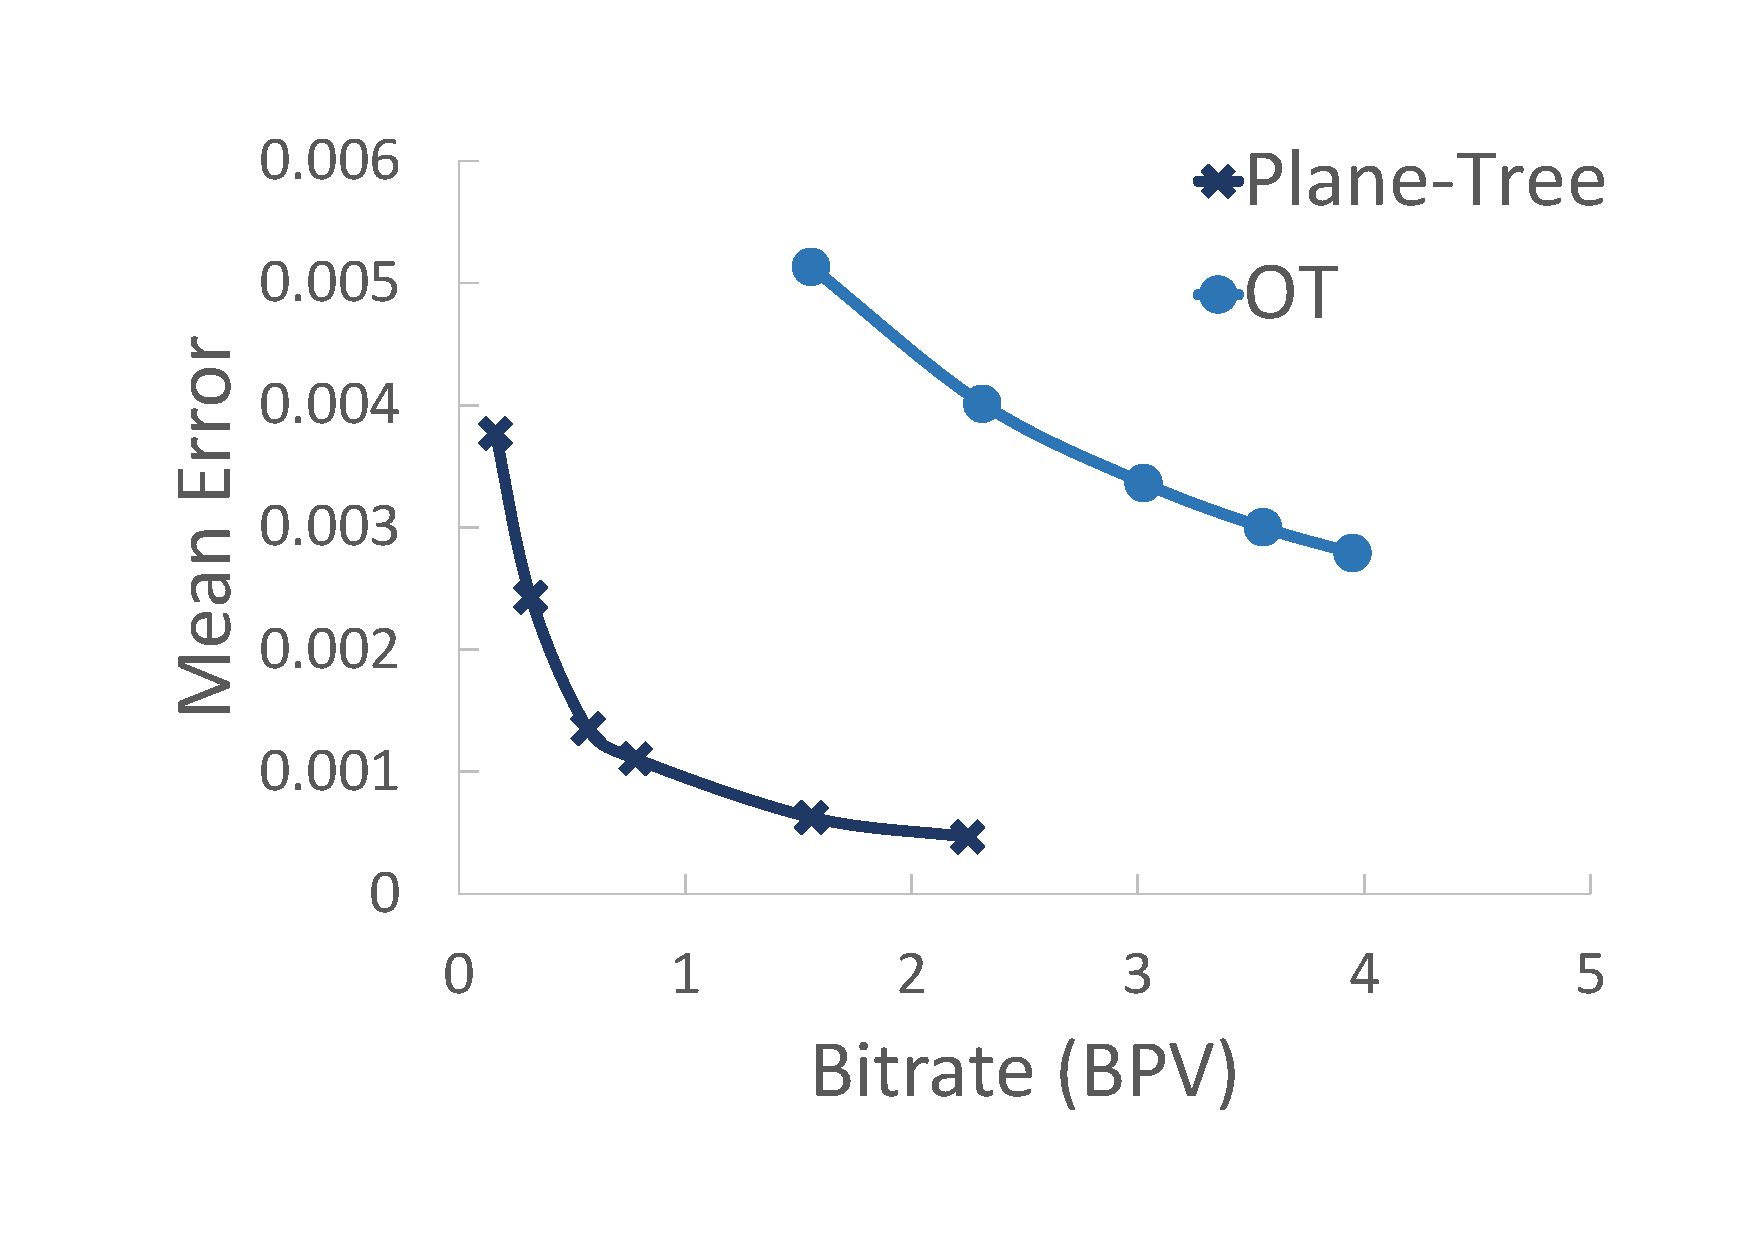
\includegraphics[width=2.5in]{images/results/compression/OTHorse}
                \caption{Horse Model}
                \label{fig:OG_HORSE}
        \end{subfigure}%

       \caption{Rate-distortion graphs comparing the Plane-Tree with the Octree.}
       \label{fig:OTEXPS}
\end{figure}

\subsection{Octree Comparisons}

Figure \ref{fig:OTEXPS} shows rate-distortion graphs comparing the Plane-Tree with the Octree compression method. In these rate-distortion graphs we use the mean error between the decoded and input model as the distortion metric. Results show that for the Bunny and Fandisk experiments (figures \ref{fig:OG_BUNNY} and \ref{fig:OG_FANDISK}) the Plane-Tree has better quality for a given bitrate compared to the Octree. It is also evident that the Octree is unable to reach the level of quality the Plane-Tree reaches. \\

In the Horse model graph in figure \ref{fig:OG_HORSE} there is some overlap in distortion levels. This shows, for a given level of quality the Octree requires around 8 times more storage space compared with the Plane-Tree. \\


\subsection{State of the Art Comparisons}

\begin{figure}[t!] 
        \centering
        \begin{subfigure}[b]{1.8in}
                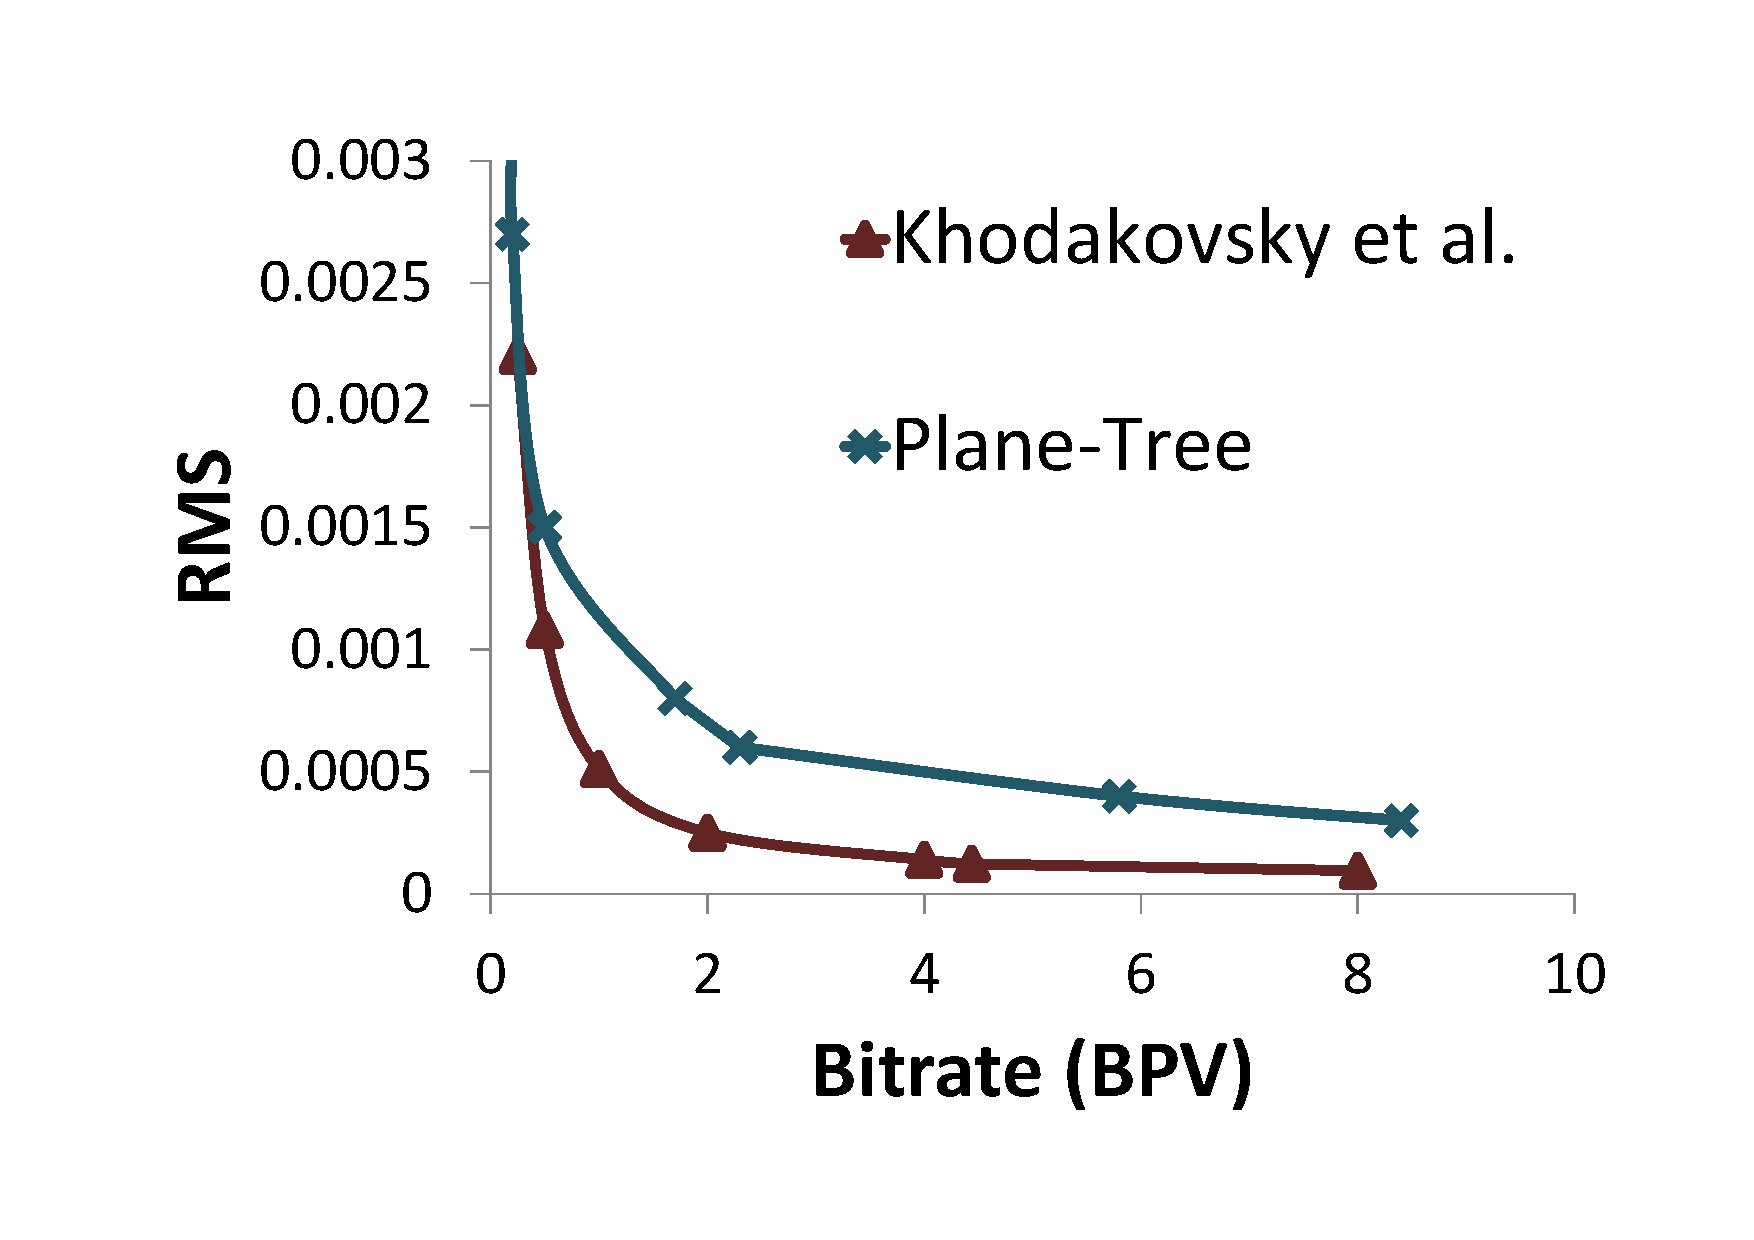
\includegraphics[width=1.8in]{images/results/compression/bunnysota}
                \caption{Bunny Model}
                \label{fig:SA_BUNNY}
        \end{subfigure}%
        \begin{subfigure}[b]{1.8in}
                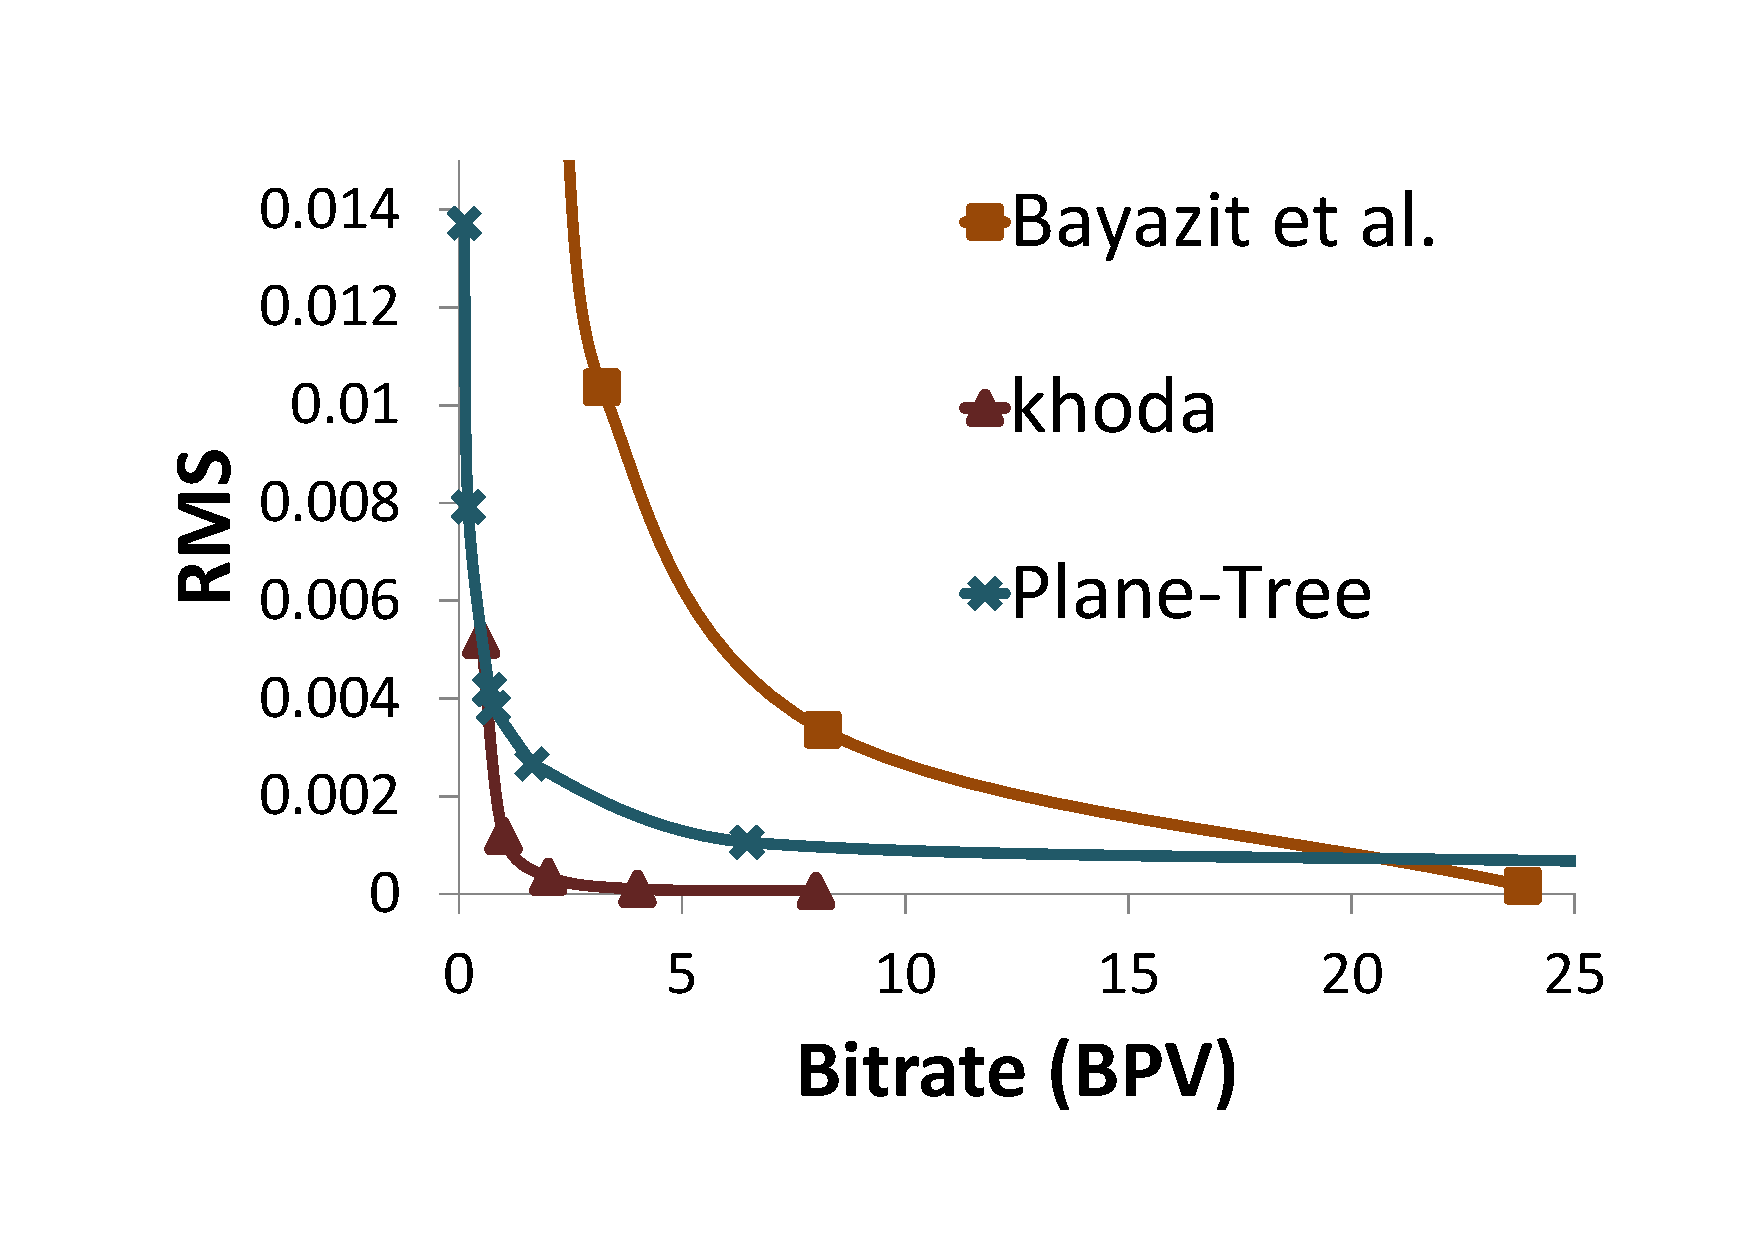
\includegraphics[width=1.8in]{images/results/compression/fandisksota}
                \caption{Fandisk Model}
                \label{fig:SA_FANDISK}
        \end{subfigure}
        
        \begin{subfigure}[b]{1.8in}
                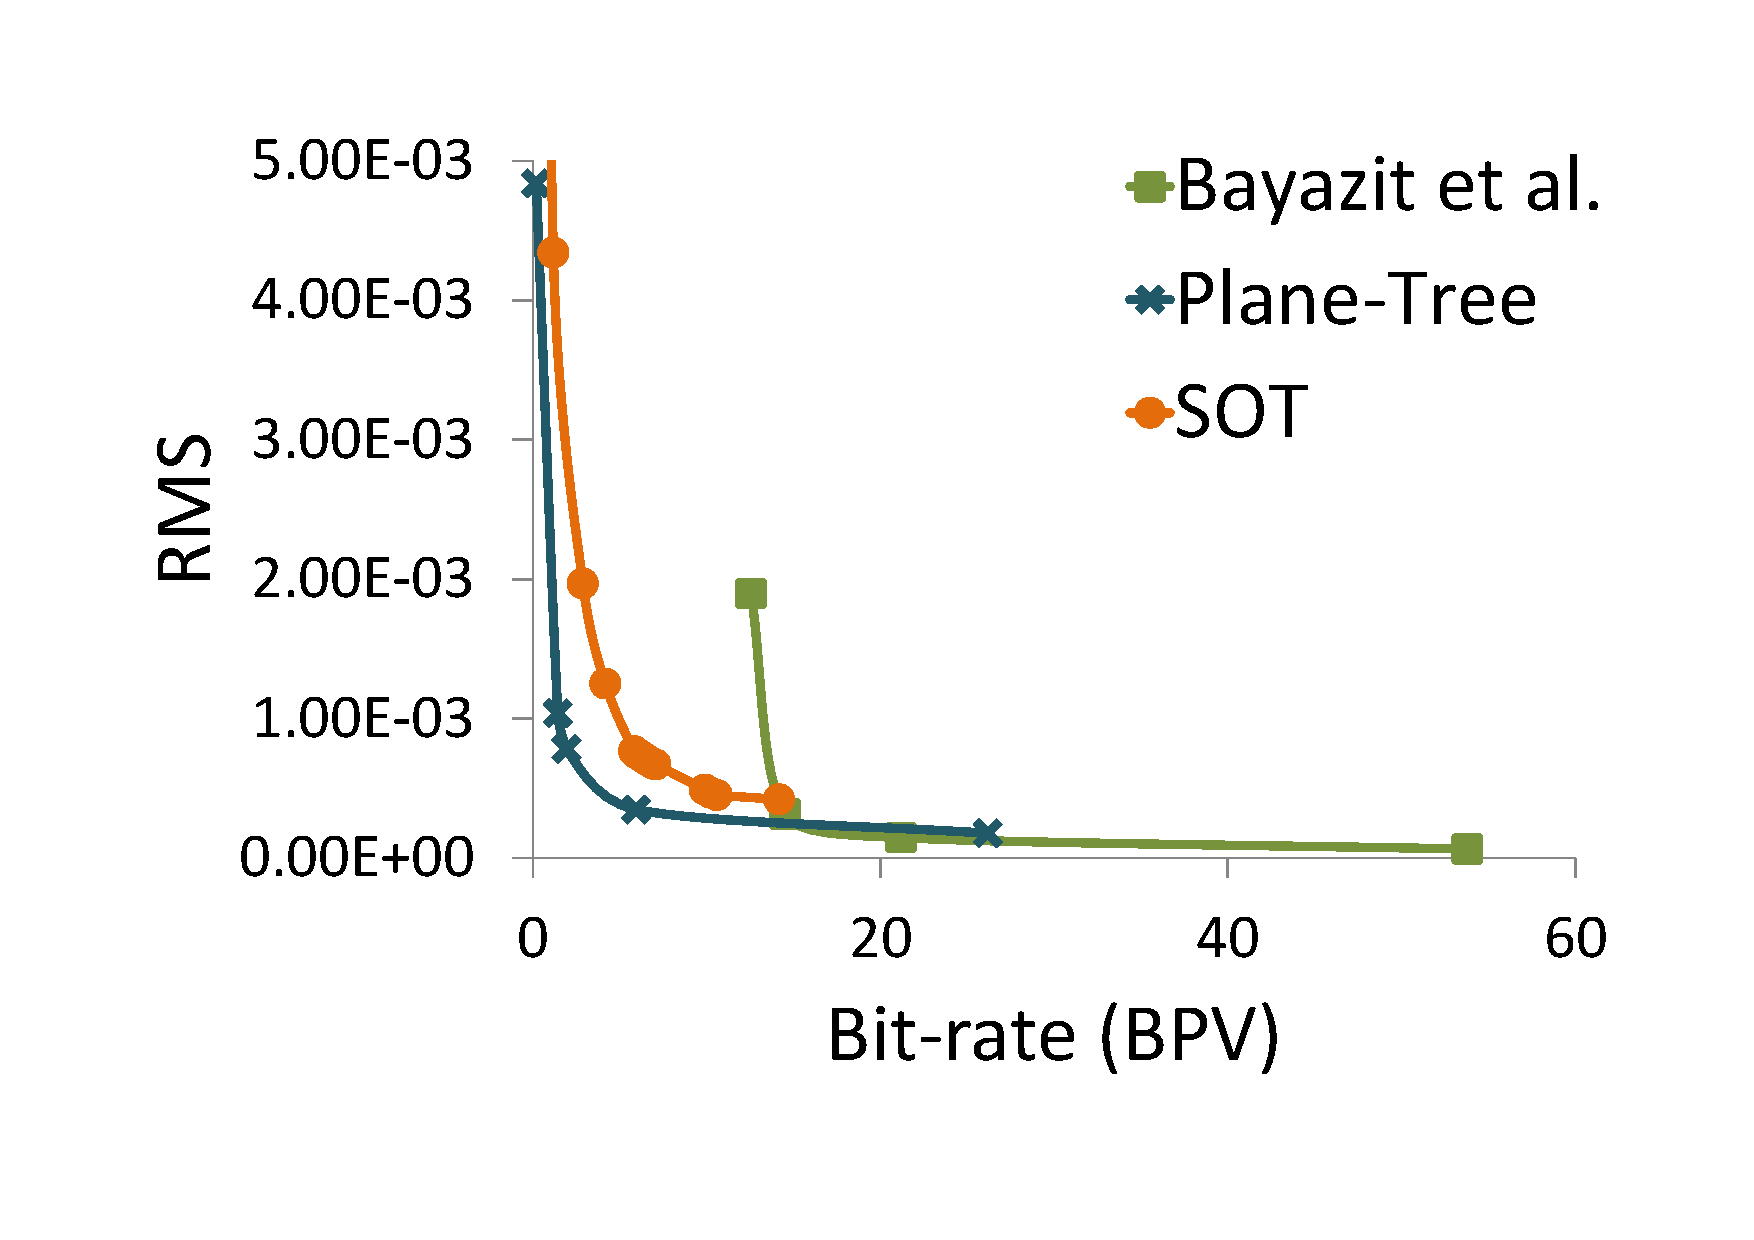
\includegraphics[width=1.8in]{images/results/compression/horsesota}
                \caption{Horse Model}
                \label{fig:SA_HORSE}
        \end{subfigure}%
        \begin{subfigure}[b]{1.8in}
                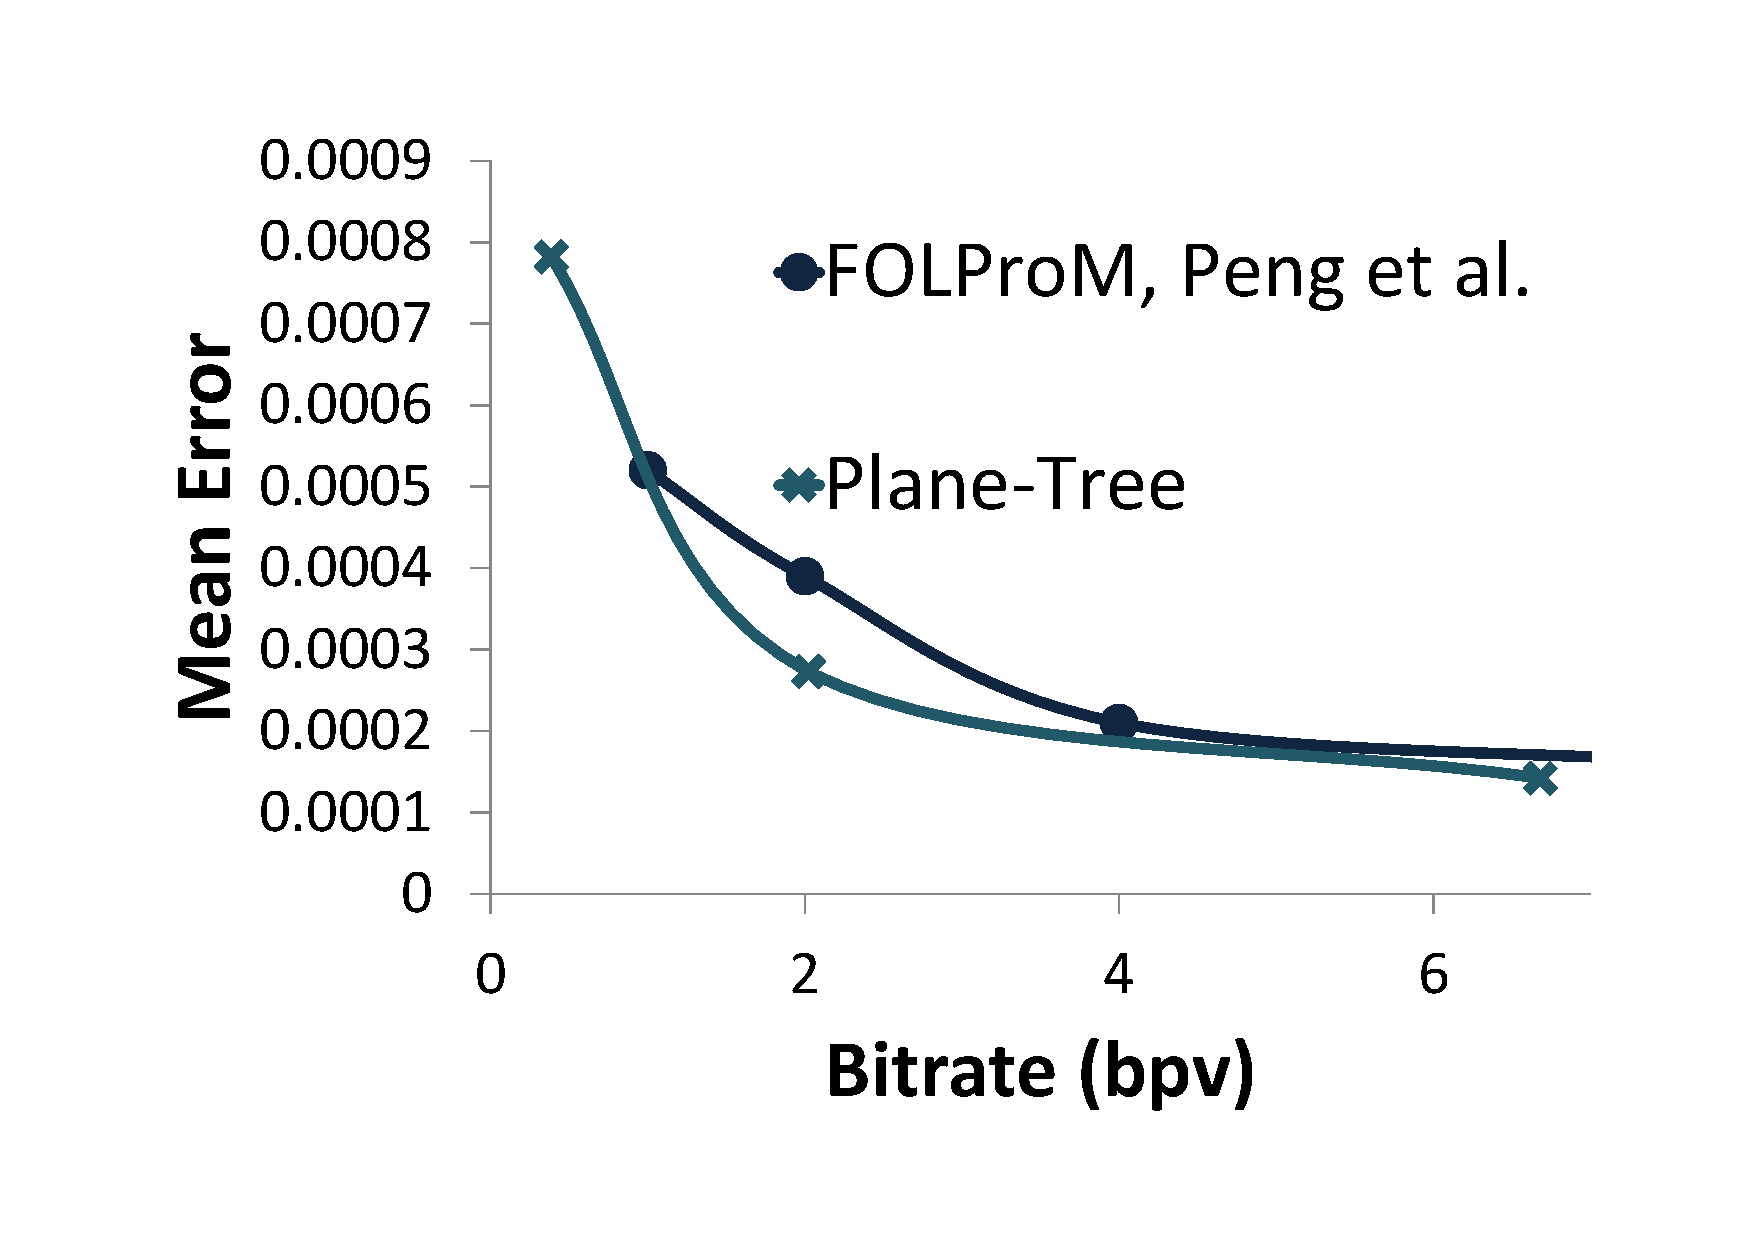
\includegraphics[width=1.8in]{images/results/compression/rabbitsota}
                \caption{Rabbit Model}
                \label{fig:SA_RABBIT}
        \end{subfigure}
       \caption{Rate-Distortion graphs comparing the Plane-Tree to different state of the art codecs.}
       \label{fig:SOTAEXPS}
\end{figure}

In figures \ref{fig:SA_BUNNY}, \ref{fig:SA_FANDISK} and \ref{fig:SA_HORSE} we compare the Plane-Tree with the state of the art transform methods by Bayazit et al \cite{Bayazit103DMesh} and Khodakovsky et al \cite{Khodakovsky00Progressive}. Figure \ref{fig:SA_BUNNY} shows the Plane-Tree has similar distortion compared with the method by Khodakovsky at low-bitrates, whilst being competitive with it up to much higher bitrates. \\

Figure \ref{fig:SA_FANDISK} shows similar results compared with Khodakovsky's method, it also shows the Plane-Tree outperforms the spectral compression method by Bayazit et al at both low and mid level bitrates. Figure \ref{fig:SA_HORSE} shows how the much simpler Plane-Tree method outperforms the transform based method of Bayazit et al. Whilst our method remains competitive at higher bitrates, it outperforms the method by Bayazit at lower bitrates. \\

Finally the Plane-Tree is compared with the state of the art low-bitrate compression system FOLProM \cite{Peng10Feature} using the mean error metric. It can be seen that at low-bitrates (below 2 bits per vertex), the Plane-Tree method outperforms this state of the art low-bitrate compression system. \\

\subsection{Qualitative Results}



\begin{figure*}[t!] 
        \centering
 		\begin{subfigure}[b]{1.9in}
                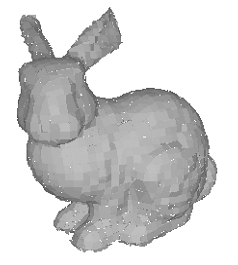
\includegraphics[width=1.6in]{images/results/compression/bunnyb}
                \caption{2.03 bpv\\8827 bytes}
                \label{fig:FIG_BUNNYB}
        \end{subfigure}%
        \begin{subfigure}[b]{1.9in}
                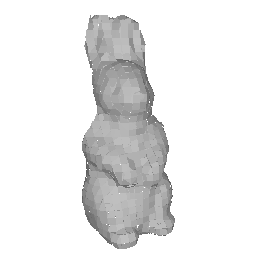
\includegraphics[width=1.6in]{images/results/compression/rabbitb}
                \caption{0.47\\3898 bytes}
                \label{fig:FIG_RABBITB}
        \end{subfigure}%
        \begin{subfigure}[b]{1.9in}
                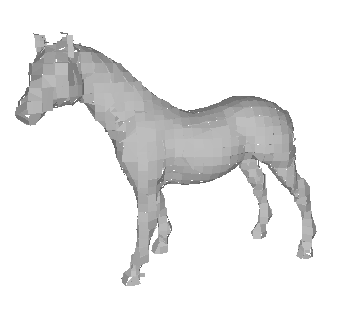
\includegraphics[width=1.6in]{images/results/compression/horseb}
                \caption{1.55 bpv\\3842 bytes}
                \label{fig:FIG_HORSEB}
        \end{subfigure}

        \begin{subfigure}[b]{1.9in}
                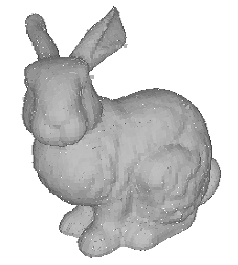
\includegraphics[width=1.6in]{images/results/compression/bunnyd}
                \caption{7.74 bpv\\33701 bytes}
                \label{fig:FIG_BUNNYD}
        \end{subfigure}%
        \begin{subfigure}[b]{1.9in}
                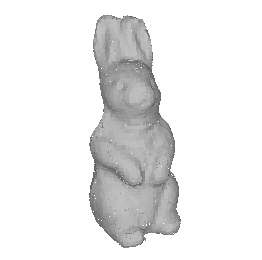
\includegraphics[width=1.6in]{images/results/compression/rabbitd}
                \caption{1.97\\16492 bytes}
                \label{fig:FIG_RABBITD}
        \end{subfigure}%
        \begin{subfigure}[b]{1.9in}
                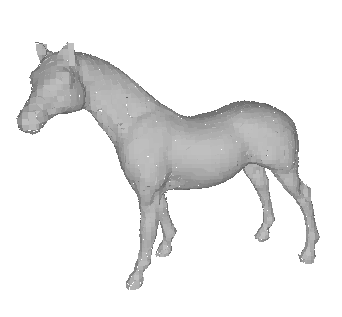
\includegraphics[width=1.6in]{images/results/compression/horsed}
                \caption{5.95 bpv\\14758 bytes}
                \label{fig:FIG_HORSED}
        \end{subfigure}
        
        \begin{subfigure}[b]{1.9in}
                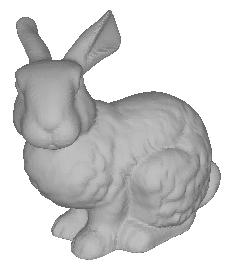
\includegraphics[width=1.6in]{images/results/compression/bunnyorig}
                \caption{original: 518.78 bpv\\2,258,902 bytes}
                \label{fig:FIG_BUNNYO}
        \end{subfigure}%
        \begin{subfigure}[b]{1.9in}
                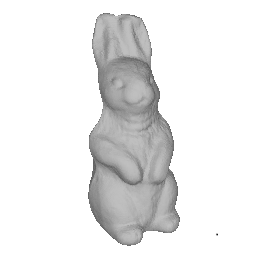
\includegraphics[width=1.6in]{images/results/compression/rabbitorig}
                \caption{original: 530.14\\4,442,413 bytes}
                \label{fig:FIG_RABBITO}
        \end{subfigure}%
        \begin{subfigure}[b]{1.9in}
                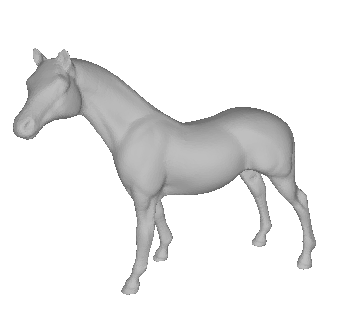
\includegraphics[width=1.6in]{images/results/compression/horseorig}
                \caption{original: 519.92 bpv\\1,290,120 bytes}
                \label{fig:FIG_HORSEO}
        \end{subfigure}
       
       \caption{Models coded with our coder at thresholds of 8.0 and 1.0 with a maximum tree depth of 6 along with the original models.}
       \label{fig:FIGS}
\end{figure*}

In figure \ref{fig:FIGS} we present qualitative results for the Plane-Tree. The third row shows the bunny, rabbit and horse models along with the number of bytes and bpv required to store them uncompressed. The first row shows each model compressed by the Plane-Tree with a threshold of 8.0. Despite these being crude approximations of the originals, the models are still distinguishable with around 1000 $\times$ less storage space required. \\

In the second row, each model was compressed with the Plane-Tree at a threshold of 1.0. In these experiments there is little detail missing compared with the physical model. When looking at the bunny's legs, the same ripples are present. In the rabbit model, the outlines inside the ears and on the eyes are still present. On the horse model, the creases on the body and shoulder of the horse are still present. Here, the bunny is compressed to around 70 $\times$ less storage space, the rabbit at around 265 $\times$ less and the horse around 90 $\times$ less storage space. \\




here we compare the volumetric plane-tree to the ot, the other methods are designed for mesh compression and since the ot is one of the most common representations used for 3d reconstruction we compare with it. we also have an implementation of ilqt extended to 3d called the ilot (interpolating leaf oct-tree) we compare with. Results show that for low bit-rates the ilot outperforms the ot. However as higher quality is required, OT outperforms this. The plane-tree which was the original envisionment of iqlt for 3D data is shown to improve upon the OT and ILOT at both low and high bit-rates. \\

\begin{figure*}[t]
\centering
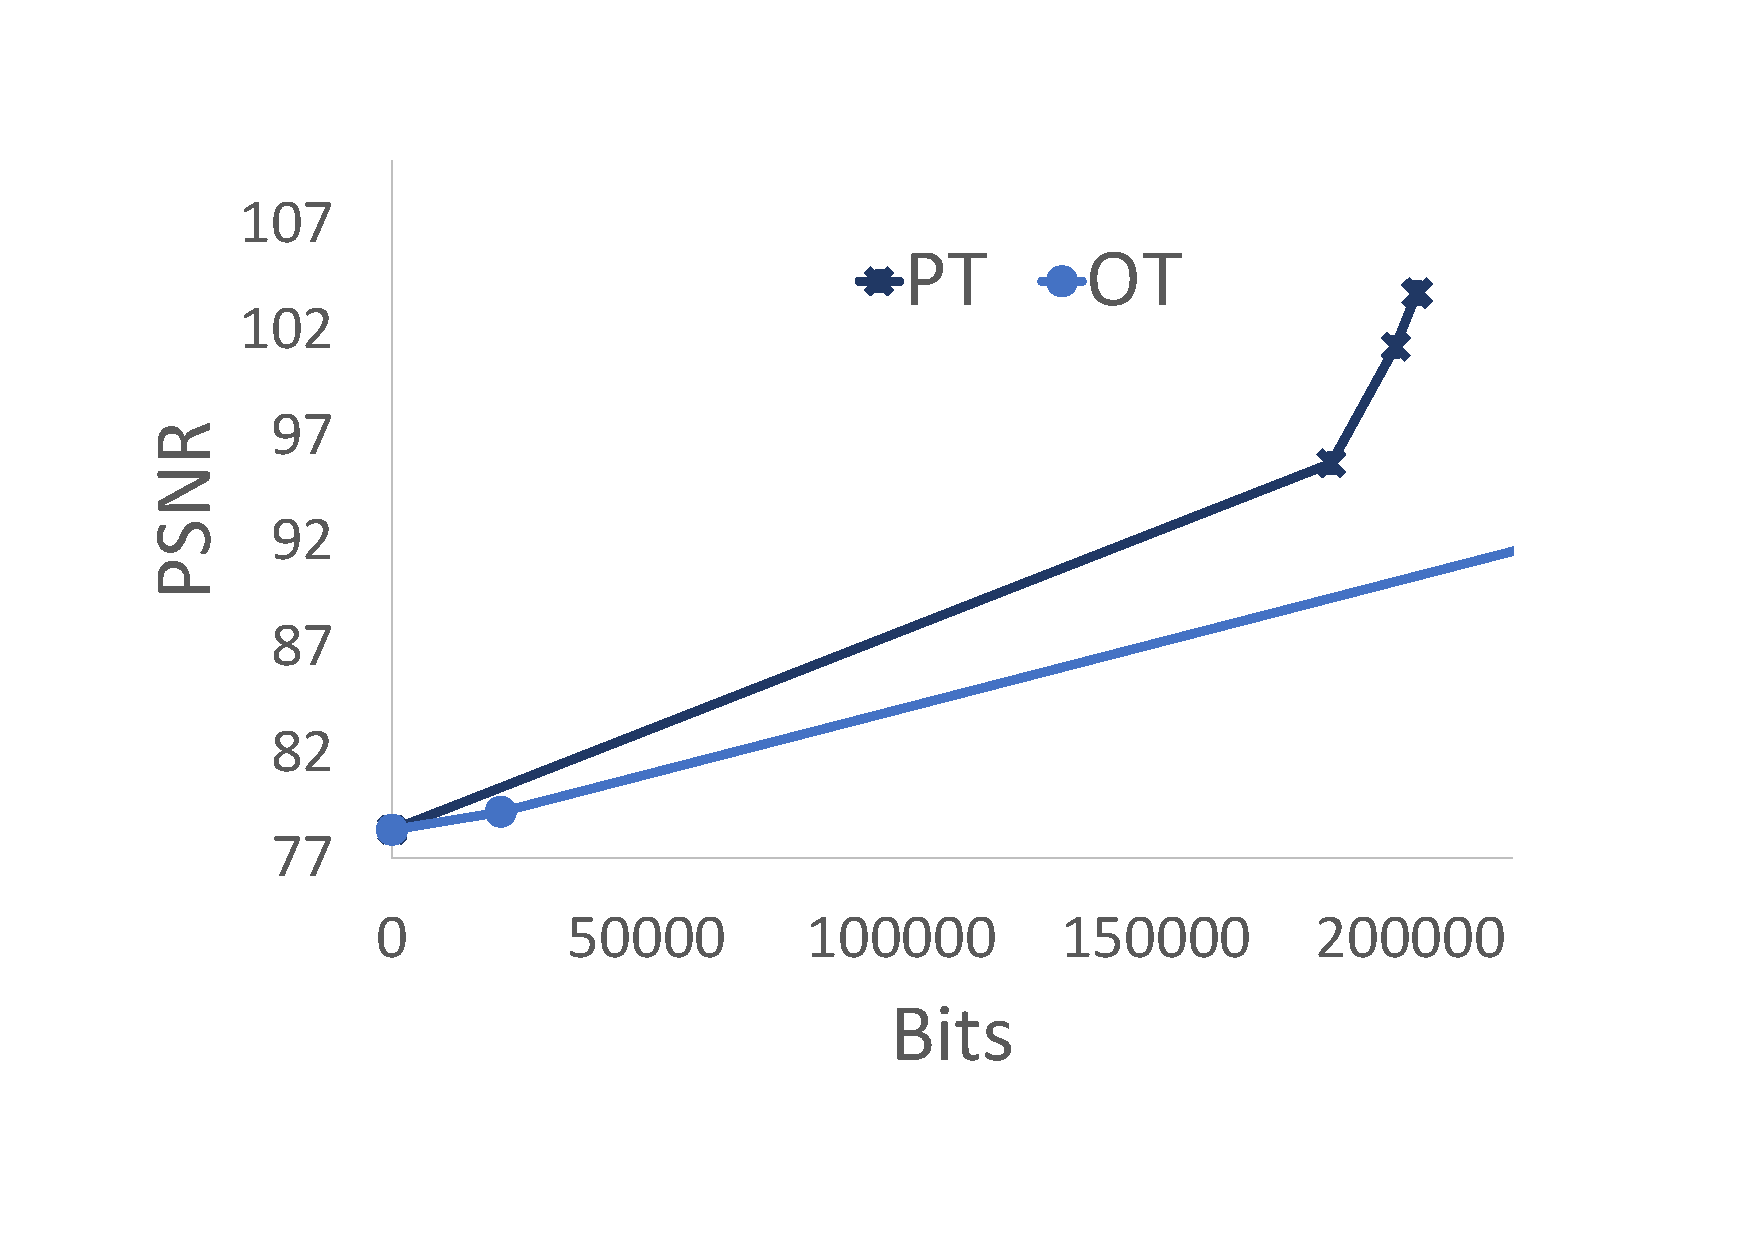
\includegraphics[width=6.0in]{images/results/compression/psnr1}
\caption{PSNR vs Bitrate comparing the ILOT, OT and PT compression methods.}
\label{fig:PSNR1}
\end{figure*}

By reducing the size of 3D reconstructions processing speed and storage will be advanced. This is advantageous in 3D reconstruction as we may want to transmit reconstructions over a network (from a robot to a base station for example). By using an advanced compression scheme we can transmit this data faster. 